
\documentclass[conference]{IEEEtran}
\usepackage{blindtext, graphicx}
\usepackage{algorithm,algpseudocode}
\usepackage{subcaption, caption}
\usepackage{amsmath}

\ifCLASSINFOpdf

\else

\fi

\usepackage{array}

\usepackage{stfloats}
\hyphenation{op-tical net-works semi-conduc-tor}


\begin{document}

	\title{Plan recovery in reactive HTNs using symbolic planning}
	
	
	\author{\IEEEauthorblockN{Lydia OULD OUALI}
		\IEEEauthorblockA{ %School of Electrical and\\Computer Engineering\\
			LIMSI-CNRS, UPR 3251, Orsay, France \\
			Univ. Paris-Sud, Orsay, France \\
			Email: ouldouali@limsi.fr
		}
		\and
		\IEEEauthorblockN{Charles RICH}
		\IEEEauthorblockA{
			Worcester Polytechnic Institute\\ Worcester, MA, USA\\
			Email: rich@wpi.edu 
		}
		\and
		\IEEEauthorblockN{Nicolas SABOURET}
		\IEEEauthorblockA{ LIMSI-CNRS, UPR 3251, Orsay, France \\
			Univ. Paris-Sud, Orsay, France \\
			Email: Nicolas.Sabouret@limsi.fr}
	}
	
	% conference papers do not typically use \thanks and this command
	% is locked out in conference mode. If really needed, such as for
	% the acknowledgment of grants, issue a \IEEEoverridecommandlockouts
	% after \documentclass
	
	% for over three affiliations, or if they all won't fit within the width
	% of the page, use this alternative format:
	% 
	%\author{\IEEEauthorblockN{Michael Shell\IEEEauthorrefmark{1},
	%Homer Simpson\IEEEauthorrefmark{2},
	%James Kirk\IEEEauthorrefmark{3}, 
	%Montgomery Scott\IEEEauthorrefmark{3} and
	%Eldon Tyrell\IEEEauthorrefmark{4}}
	%\IEEEauthorblockA{\IEEEauthorrefmark{1}School of Electrical and Computer Engineering\\
	%Georgia Institute of Technology,
	%Atlanta, Georgia 30332--0250\\ Email: see http://www.michaelshell.org/contact.html}
	%\IEEEauthorblockA{\IEEEauthorrefmark{2}Twentieth Century Fox, Springfield, USA\\
	%Email: homer@thesimpsons.com}
	%\IEEEauthorblockA{\IEEEauthorrefmark{3}Starfleet Academy, San Francisco, California 96678-2391\\
	%Telephone: (800) 555--1212, Fax: (888) 555--1212}
	%\IEEEauthorblockA{\IEEEauthorrefmark{4}Tyrell Inc., 123 Replicant Street, Los Angeles, California 90210--4321}}
	
	
	
	
	% use for special paper notices
	%\IEEEspecialpapernotice{(Invited Paper)}
	
	
	
	
	% make the title area
	\maketitle
	
	%	
	\begin{abstract}
		Hierarchical reactive methods are very popular in the field of controlling complex artificial intelligent	agents in dynamic environment. However, dynamic environments are incompletely known and can change in unpredictable way which make the planning systems fail. In this paper,  we describe a hybrid planning system called \emph{Discolog} which extends a reactive planning system  with a linear symbolic planning system  to propose a strategy to recover from breakdown.   Our solution has been implemented on the reactive system \emph{Disco} which been extended with the symbolic planning system STRIPS. 
			
		
	\end{abstract}
	\IEEEpeerreviewmaketitle
	
	
	
	\section{Introduction}
	\par Using automatic planning systems in real world applications is a three process. First, the system designer has to build a formal representation of the world called \emph{domain knowledge} that reflects the realty .Second, the system has to reason about this domain knowledge and produce a sequence of actions. Third, The system should monitors the success  of the computed plan execution in the real world.  each element of theses three elements depends on the others. Thus, if the domain knowledge is poorly designed, then, plans produced from such domain knowledge might go wrong during the execution.  
	\par 	In this context , AI researchers have developed two complementary approaches to  construct planning systems. 
	\par The first approach is symbolic planning. This approach consists in constructing a logical description of the world to compute  off-line a full plan to achieve agent's goals.  Their exist a variety of architecture using this approach. The most popular one is called HTN (i.e Hierarchical Task Network) \cite{erol1996hierarchical}. HTNs allow a recursive decomposition of complex goals into sub-goals or primitive actions. This architecture eases the design of the world and gives more expressiveness. However, the plan execution in the real world might drift from what was planned off-line and make the execution fail. For example, imagine an agent that plans to move a box from \textit{Room 1} to \textit{Room 2} through an opened door \textit{Door}. The HTN representation of the example is depicted in figure \ref{Fig:repair}. After executing the task \textit{Pick up(Box)}, the agent attempts to execute the task \textit{Walk(Room1, Room2)}, but during the execution, the wind blows and  the door closes. Then, when the agent tries to execute the \textit{Walk} task, it fails. Such situation is called a \emph{breakdown}; it is caused by the dynamic nature of the environment. Symbolic planning thus faces two difficulties. First, authoring an exact representation of a dynamic and complex world requires significant  knowledge-engineering effort \cite{zhuo2009learning}, and even reveals to be impossible \cite{maes1990designing}. However, with incomplete knowledge the agent cannot anticipate the future and the generated plan might be not executed as expected. Second, symbolic planning assumes that the world can only be changed by the agent actions. However, dynamic world can be modified  by external participants such as the wind in the example \ref{Fig:repair} and other agents evolving in the world.  	  
	\begin{figure}[t]
		\centering
		\frame{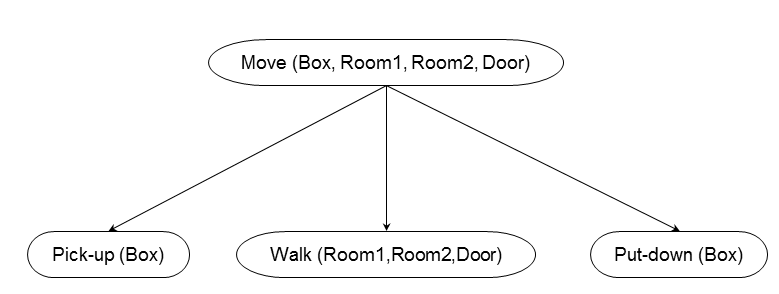
\includegraphics[width= \columnwidth]{Figures/repair.png}}
		\caption{HTN decomposition of the Move Box task}
		\label{Fig:repair}
	\end{figure}
	\par The second approach is called  reactive planning \cite{firby1987investigation}.It gives up on long-term prediction since the world is too dynamic to be anticipated. It leaves all the planning during the execution phase: the agent plans only for the next step to be executed from the current  state of the world. Thus, it can adapt the goal decomposition and action selection according to the observed changes in the world. For this purpose, reactive planning utilizes procedures (a.k.a procedural knowledge) to the execution and goal decomposition. The main advantage of procedural knowledge is that it is closer and more representative to the real world which reduce the complexity of planning and still can cope with complex dynamic environments \cite {brom2005hierarchical}. However, procedural knowledge is limited, it is defined as black-box procedures (for example : JavaScript code) that  can only be executed, while symbolic knowledge allows reasoning about actions and inference. 
	\par Reactive planning generally uses the same hierarchical architecture as HTNs \cite{erol1994htn}. Complex goals are thus decomposed in subgoals until atomic goal are reached. Therefore, we resume in our work hierarchical reactive planning to reactive HTN.
	Reactive HTNs are used in numerous application domains, such as dialog systems \cite{bohus2003ravenclaw}, games \cite{isla2005handling} and simulating human behavior \cite{brom2005hierarchical}. 
	\par During the execution \emph{breakdowns} can  appear because the execution leads a state where no possible action can be executed next. It can occur because the execution of the precedent action fails, or a change occurs in the world and bring it to a dead end state.  In such situation, the agent has to stop and think of a strategy to reach its goal. Reactive HTNs are unable to construct a plan repair to recover from breakdowns for two main reasons. First, reactive planning don't use long term prediction. It is not able to construct a plan based on a projection into the future states of the world. Second, procedural knowledge is defined with any logical information to allow the HTN reason about the breakdown and  eventual plan recovery.
	
	\par In this work, we claim  that with a minimum definition of symbolic planning, agents can build efficient local plans to recover from breakdowns. To that end, we analyzed the procedural knowledge to figure out that procedural task's operators defined in the reactive HTN domain knowledge are, for the most of them boolean procedures which can be thought as logical predicates. Therefore,  we first propose to the HTN designer to convert theses procedures to a symbolic knowledge to have a support for reasoning. Second, we propose to monitors the execution and build a module to recover from breakdowns. Since reactive HTNs cannot reason on theses knowledge, we  extend  reactive HTN  with a linear symbolic planner  to compute plans recovery.  We study the capacity of such hybrid model to support a hybrid domain knowledge to recover from breakdowns in dynamic environment.	
	
	\par Section 2 present an example to explain our motivation. Section 3 briefly presents existing works in this domain. In section 4, we formalize the proposed solution \textit{Discolog}. In section 5, we first  describe the \textit{Discolog}. implementation. Next, we present the preliminary evaluation to our model. We discuss the obtained solutions and the impact of both quantity and quality of the extracted symbolic knowledge in the recovery process.
	\section{motivation example}
	This section illustrates a simple real-world example that will make our motivation and proposition clearer. lets consider a robot responsible for charging object into trucks. The  goal task decomposition to achieve the load task is described in Figure \ref{fig:ex}.

	\label{sec:example}
	\begin{figure*}[t]

	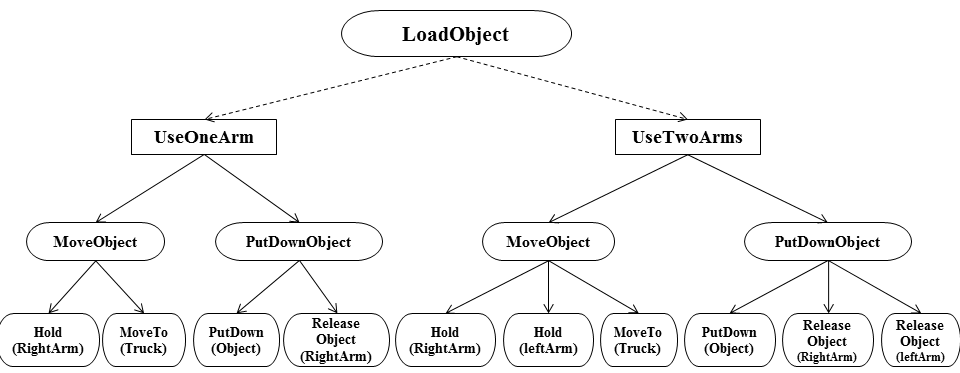
\includegraphics[width=\textwidth]{Figures/example}
	\caption{Load Object task decomposition for robot arm motion}
	\label{fig:ex}
	\end{figure*}
 
			
	\par To load an object into the truck, the robot has to move it from its initial place and put it into the truck. The agent starts by decomposing the goal task "LoadObject". This task is defined with two recipes to manipulate the object. Depending on the object's  weight, the robot will choose the corresponding recipe as described in figure \ref{fig:ex}: the first recipe proposes to use one arm if the object's weight is below than 5 kilograms. The second recipe proposes to use both of the robot arms if the weight of the object is higher than 5 kilos and below than 10 kilos. Once the robot chooses the recipe, it has next to perform  its corresponding tasks; "MoveObejct" and "PutDownObject", which are decomposed into primitive tasks that are executed in the real world. 
	\par If we consider now an object with the weight of 20 kilos. The "LoadTask" execution is  performed as follows: The robot attempts to decompose the "LoadObject" task. It has thus to choose which recipe perform.It invokes a sensor to calculate the object's weight. It tries to perform the first recipe, but the object is heavier than 5 kilos which contradicts the script of the applicability condition and make this recipe inapplicable. Therefore, it tries the second recipe "usetwoArms" and holds the object with both of its arms but it fails again because the object is heavier than 10 kilos which make the applicability condition of the second recipe also fails. At this moment, all the available recipes to decompose the "LoadTask" task are inapplicable. At this point, the execution is blocked with no possible task to execute. A breakdown is then reached by the robot. 
	\par When a breakdown is detected, the robot has to think of a strategy or a plan to get out from this breakdown.  In  section \ref{solution} we present our proposition to overcome the breakdown problem. But before, we present the background related to our work. 

	\section{Background and related works}
	Basic requirements to build planning systems is to have a formal representation of the environment (i.e domain knowledge) and planning engine to reason about this knowledge. Several approaches have been proposed for this purpose. 
	
	\subsection{Symbolic planning}
	\label{sec:symbolic}
	The first contribution in planning was symbolic linear planning systems (STRIPS)\cite{fikes1972strips} which model the environment as a set of actions and transitions between those actions . Linear planning attempt to generate a plan (i.e. a sequence of actions) which once executed transform the initial state of the environment to a final state where the agent goal is achieved. 
		
	\par Due the complexity of planning problems description, HTN (Hierarchical Task Network)  \cite{erol1996hierarchical} was proposed. 	
	HTN domain knowledge can be represented as AND/OR tree. AND nodes represents tasks. each task is defined with preconditions to check the applicability of the task and postconditions  that checks the success of the task execution. There are two different types of tasks: primitive tasks (leaf nodes) are similar to linear planning actions which can directly be performed in the environment. Compound tasks have to be decomposed into subtasks using a corresponding recipe. Recipes of tasks are defined as OR nodes and represent a method of decomposition of compound tasks. each recipe has  applicability conditions.
	\par  HTN planners intent to plan for one or more goal task. Planning proceeds using task decomposition that decomposes goal task  using a corresponding recipe into a sequence of simpler subtasks. This process is applied recursively until a conflict-free plan (sequence of primitive tasks or actions ) that can make the goal task successful is found. 
	HTN planners become popular this last decade  where several systems were developed such as SHOP \cite{nau1999shop}, SIPE \cite{wilkins1988practical} or NOAH  \cite{sacerdoti1975structure}. 
	\par During the execution in a highly dynamic environment, an action execution might drift from what was expected because of the lack of information about all the changes in the environment. Such situation causes an execution failure or \emph{breakdown} and the planner can no longer achieve its goal. 
	Several researchers in symbolic planning have been attacking this problem by integrating a plan repair module \cite{boella2002replanning, van2005plan,hayashi2006dynagent,ayan2007hotride,warfield2007adaptation}. Thus, if a breakdown is detected, the plan repair module uses a causal graph that contains all the logical dependencies between the HTN task  to calculate the task candidate to repair (the strategy for computing the task candidate differs). Next, the planning system is called again to propose a new decomposition to the  task candidate.
	The presented solutions avoid replanning from the scratch and proposes a local repair with minimal costs. However, they presents some limitations. first, the plan repair remain dependent to the initial planning system. Thus, if this latter is unable to find a plan repair, then the HTN definitively fails to achieve the goal. Second, theses systems inherit the limitations of symbolic planning: with limited knowledge, the HTN can not always find other decompositions to tasks. Finally,  These solutions are only applicable for the HTN they trying to repair. In addition, the plan repair solutions can not be generalized to reactive HTN, they exploit  logical dependencies to calculate the task candidate which make them and are impossible to apply in reactive HTN due to the absence of logical knowledge in procedural formalism.
	\subsection{Reactive planning}
	
	\par The problem of planning in highly dynamic environment with incomplete knowledge has been tackled in reactive planning systems \cite{schoppers1987universal}. 
	Reactive planning systems have two main characteristics. The first is the hierarchical tree-like structure of the planning system which is similar to HTNs. in the following we will name  "Reactive planning systems" directly "reactive HTNs".
	The second is that HTN planning avoids long term prediction. Instead, it plans only for the next act to perform at every moment which allows reactive HTN adapting its next act to the observed changes in the real environment. Therefore, action execution is not selected from a pre-constructed plan but it is computed directly in the execution process.
	Actions to perform are selected from a hand coded domain knowledge proposed by the planner designer. Instead of modeling the environment, reactive HTNs attempt to model the policy of the agent in its environment (i.e all the tasks that it can perform). In addition, action's operators don't contain any logical information and are represented as simple code procedure (for example JavaScript, XML). Thus, the planner cannot reason about this knowledge. This type of domain knowledge is called \emph{Procedural domain knowledge}.
	\par Reactive planning becomes very popular in AI and for most of cases uses an HTN formalism to model their domain knowledge. For instance, in Robotics where \cite{firby1987investigation} defends a parallel reactive architecture with \emph{Reactive Action packages} representing autonomous process used to achieve the different goals of the robot. \cite{bryson2001intelligence} and \cite{brom2005hierarchical} propose a reactive planning system for prototyping human-like behavior in a virtual environment to ensure a natural behavior with respect of time constraint and reactivity with the real world. Reactive planning is also used in Gaming with the name of  behavior trees \cite{isla2005handling}. Behaviors trees have the same hierarchical structure of HTNs and do real time decision which can be seen as reactive planning. 
	
	
	\par Reactive planning also rise the problematic  of \emph{breakdowns} among researchers dealing with investigations in reactive planning. The work presented in  \cite{firby1987investigation} suggests that robots need strategic planning to detect problematic situations before they occur. Therefore, it proposes to add a strategic planner's job which put constraints on the planner behavior before its execution in order to prevent inefficiencies. Theses constraints can be an ordering tasks in the execution queue of the planner or choosing the most promising decomposition for compounded tasks.
	
	C.Brom \cite{brom2005hierarchical} discussed the observed limitations of the  Hierarchical Reactive planning (HRP) used to control human agents or IVAs (Intelligent Virtual Agent) that degrade the believability of the IVA behavior. Among the limits discussed in his work, he discussed the necessity of planning to maintain believable and intelligent behavior of the agent. For example to be able to see the distance of its tasks especially to achieve goals with time constraint. to . To overcome these limitation,HPR's execution was extended by a semantic StateFull plans (SPF) and the resulting architecture is named StateFull HRP \cite{plchtowards}.  SPF is a Finite State Machine that integrate HRP's reactive plan as part of its workflow. In addition, a semantic layer is added to allow the agent reasoning, planning and cleaning up its behavior. The results of this architecture is a more structured plan execution that ensure a more believable behavior of IVA.   
	\par In this paper we support the claim of strategic planning to extend reactive planning. Therefore, we present a different approach based on a hybrid system that extends a reactive planning system with a symbolic planner to recover from breakdowns. This solution is simple to implement and can be generalized to different reactive HTN's architecture. 

	
	
	\section{Hybrid model: Extending reactive HTNs with symbolic planning}
	\label{solution}
	\par We address the problem of breakdown  by extending reactive HTNs with symbolic linear planner that construct local strategies to recover from the faced breakdowns.
	The produced hybrid system combines HTN's reactive knowledge, and the symbolic knowledge of linear planning systems.
	\par To construct the symbolic knowledge requisite to  linear planner for reasoning. We propose to  extract it directly from the HTN's reactive knowledge. Reactive knowledge is mostly made up of boolean procedures which can be thought as logical predicates. We propose thus to the HTN desinger to extend these boolean procedures into  symbolic knowledge. In addition, linear planner reasons only on primitive tasks (i.e actions) (see section \ref{sec:symbolic}), then the knowledge extraction will be focused on primitive tasks with boolean structure.


  %\begin{figure}
  \begin{algorithm}
  	\begin{algorithmic}[1]

  	\caption{ Reactive planning and plan recovery algorithm}
  	  				\label{pseudoPSO}
  		\Procedure{Hybrid system}{$DomainKnowlege,Goal$}
  		\State $\pi \gets Reactive HTN \textit{(DomainKnowlege,Goal)}$
  		\If{$\pi = \textit{Success} $}
  		\State \Return $\textit{Success} $
  		\EndIf
  		\State {$plan \gets Recover(Goal)$}
  
  		\If{$plan = \textit{null}$}
  		\State \Return $\textit{Failure} $
  		\EndIf
  			\ForAll {$action$ $a_i \in plan$}
  			\State $\textit{Discolog} (HTN,a_i) $
  			\EndFor
  		
  		\EndProcedure
  		
  		\Procedure{Recover}{$Goal$}
  				\State $ Candidates\gets\textit{findCandidate}{(G)} $
  				\If {$ Candidates = \emptyset $} 
  				\State \Return $null $
  				\EndIf
  
  		\ForAll {$candidate \in Candidates$}
  			\State $\Pi +=  LinearPlanner(candidate, CS)$
  				\State \Comment $CS$: current state of the world
  		\State  $Cost \gets \{ cost(\pi) | \pi \in  \Pi \} $
  		\EndFor
  		
  		\State \Return $\pi \in \Pi$  with minimum $cost(\pi)$
  		\EndProcedure
  		
  		\Procedure{FindCandidates}{$Goal$}
  			\ForAll { $child \in Goal$}
  			\If {$precondition(child)!=\emptyset$ $ and$ $\textit{status} (child)\notin\{Done, Live, Blocked\})$}
  				\State add precondition(child) to Candidates
  			
  				\ElsIf{ $postcondition(child)!=\emptyset$ $and$ $\textit{ status}(child)\in\{Failed\}$}
  				\State add postcondition(child) to Candidates
  			\EndIf
  				
  			\If  { $\textit{status} \in \{Live\}$ $and$ $nonPrimitive(child)$ $and$ $applicability(child)!=  \emptyset)$}
  				\State add App-condition(child) to Candidates
  			\EndIf
  			\State $\textit{findCandidates} (children(child))$
  			\EndFor
  			\State\Return Candidates
  			
  			\EndProcedure 
  		
  	\end{algorithmic}
  \end{algorithm}

\par Our algorithm outlined in algorithm \ref{pseudoPSO}, performs first the reactive HTN to achieve th goal. The world is monitored at each step of the execution to check the success of the HTN execution. However, breakdowns might occur and make the  HTN execution fails. 

	\par When a breakdown is detected, the algorithm invokes the \textit{recover} procedure. First, it traverses the hierarchy of the goal task to detect all its children tasks affected by the breakdown. A task is considered as failed if one of its conditions are no longer valid. Thus, the algorithm computes a list of task's failed conditions called \textit{Candidates}, using for that the task's status. A task status can be \textit{Live} (Task preconditions are valid and the task can be performed), \textit{ Done} (The task has been executed successfully),  \textit{Failed} (Task execution failed) or \textit{Blocked}  (Task preconditions are not valid). The candidates search is carried out by the sub-procedure \textit{FindCandidates}  which add a task's preconditions as candidate if its status is  \textit{Blocked}, or its postconditions if its status is \textit{Failed}.	 If the task is a compound task with its status to \textit{Live} and none of its recipes are valid then the applicability conditions of those recipes are considered as candidates.

	For instance, taking back the example described in  section \ref{sec:example}, a breakdown is detected because no recipe can be applied to decompose the "LoadObject" task. The system, then calls the recover procedure to detect all the affected tasks by this breakdown. The \textit{Candidates} list includes both applicability conditions of the failed recipes, the postconditions of the task and the "LoadObject" task. Note that a condition is considered as candidate only if it can be converted to a symbolic formalism. Otherwise, the recover procedure ignores this condition. 
	
	\par Once the \textit{Candidates} list has been determined, the linear planner attempts to propose a plan for each candidate. As linear planners plan to reach a state rather than achieving goal tasks, then each conditions candidate \textit{Candidates}  is considered as goal state to reach.  The linear planner plans  for each candidate and tries to return a list of possible plans $\Pi$ to recover from the breakdown. The most promising plan in $\Pi$  is returned by the algorithm to be executed. We define the most promising plan as the shortest plan (i.e the plan that contains the less actions) to ensure local task repair and prevent other breakdowns due to the execution of pre-constructed plan. Thus, in the example, the recover procedure returns a plan that repair the failed recipe "HoldWithTwoArm". The proposing plan  consists on using a, existing task "Separate the Object" to separate the object into two objects of 10 kilos and load them separately.
	
	\section{Implementation and experimental results}
	\subsection{Discolog implementation}
	\par The proposition discussed in this paper has been implemented using a reactive HTN called  Disco \cite{rich2009building} and a simple linear STRIPS planner, the STRIPS version used in this system is an existing  Prolog implementation proposed in \cite{poole1998computational}. Thus, we named the produced system \emph{Discolog}. 
	\par  Disco uses the ANSI/CEA-2018 standard for the procedural definition of its domain knowledge and a Java-based reactive planning system. Tasks are modeled using the XML format. Primitive tasks contain grounding script parameter defined	as JavaScript programs which represent the effect of  primitive task execution in the environment. 
	\par  The integration of STRIPS in the Disco system is performed using  \emph{tuProlog} \footnote{http://apice.unibo.it/xwiki/bin/view/Tuprolog/} framework. The use of  \emph{tuProlog} presents two mains advantages. First, \emph{tuProlog} is a Java-based framework that exploits a Prolog engine directly from a Java program. Thus, STRIPS can locally raised without any call to an external system. Second, it has specific libraries for  Prolog predicates that eases the conversion of recovery candidates from the procedural knowledge to symbolic knowledge. 
	\subsection{Experiments and results}
	\par  In this section, we present ou experiment with the \emph{Discolog} system. The aim of this  experiment is first to validate the hybrid architecture of Discolog system. Second, we want to test the contribution of the symbolic knowledge in the performances of recovery. We make the assumption that the effectiveness of the recovery process is relied to the level of knowledge in the symbolic domain knowledge. In fact, we assume that the more information STRIPS planner gets from the procedural domain knowledge, the more effective recover plans it can generates. The result of this experiment should proves that plan recovery follows a monotonic evolution in function of the level of knowledge defined in STRIPS.
	
	\par In order to validate  Discolog, we had to test it on different HTNs domain knowledge and analyze its ability of recovery on every possible breakdown. Nevertheless, in the absence of accurate models including reactive and symbolic knowledge, we  implemented our own evaluation data. 
	\par As theses primary tests purpose is to validate the hybrid architecture of Discolog, we actually don't need a domain knowledge with a semantic description of its tasks. Therefore, we defined a procedural domain knowledge based only on synthetic data  structured in such way to ensure a believable execution.  Each compound task is defined with a set of recipes and each recipe is constituted by a set of children tasks to decompose the parent task. Preconditions of compound task are propagated to its first child in each recipe, and the postconditions are propagated to its last child. 
	The rest of task children in each recipe are defined with chained conditions: The postconditions of the $task_i$ activate the preconditions of the $task_{i+1}$. Symbolic knowledge is extracted from the procedural one. Depending on the level of knowledge we want to study, we randomly extract primitive tasks from the HTN procedural knowledge.   The goal is to study the affect of the level of symbolic knowledge defined on recovery.
	\par We tested Discolog on different HTNs model. We denote ($\alpha$, $\beta$, $\gamma$)  respectively the depth of the HTN, number of recipes per each task, number task children per recipe. For each HTN, we varied first, the level of symbolic knowledge to be extracted \{25\%, 50\%, 75\%\} \footnote{0 \% of symblic knowledge means no possible recovery and 100 \% is not realistic taking in account the dynamic definition of environment}. For each level of knowledge, we randomly extracted different symbolic domain knowledge.  Second, the initial state is randomly defined. This later affects the decomposition that the HTN will choose and the plan recover procedure. 
	Once theses parameters are set, for each primitive task, a breakdown is caused and the plan recovery for this task is analyzed. The experiments have been done on two different HTN configuration as presented in table \ref{table}.
	\begin{table}[h]
		
		\centering % used for centering table
		\caption{Configuration of the HTNs } % title of Table
		\begin{tabular}{|c|c|c|c|} 
			\hline
			Configuration & Total Nb of nodes & Init state & Nb of symbolic DN\\
			\hline
			(3,3,3) & 91 & 10 & 60  \\
			(5,1,4) & 341 & 10 & 60  \\
			\hline
		\end{tabular}
		\label{table} % is used to refer this table in the text
	\end{table}
	
	
	\begin{figure}[t]
		\centering
		\begin{subfigure}[b]{0.5 \columnwidth}            
			\frame{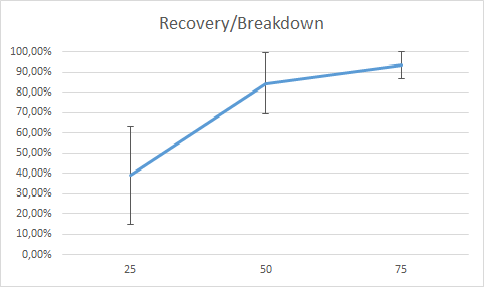
\includegraphics[width=6cm]{Figures/3.png}}
			\caption{ Recover rate for each level of knowledge}
			\label{Fig:Data3}
		\end{subfigure}
		%
		\hspace{1cm}
		%
		\begin{subfigure}[b]{0.5 \columnwidth}
			\centering
			\frame{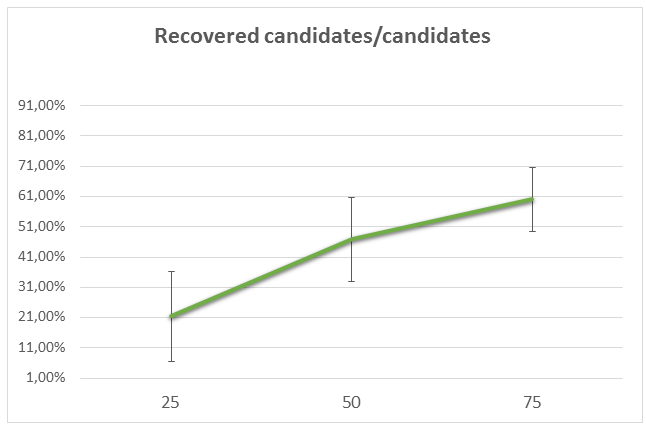
\includegraphics[width=6cm]{Figures/4.png}}
			\caption{Average number of candidates repaired for each level of knowledge}
			\label{Fig:Data4}
		\end{subfigure}
		\caption{Results for the (3, 3, 3) HTN}\label{fig:TOF}
	\end{figure}
	
	\begin{figure}[t]
		\centering
		\begin{subfigure}[b]{0.5 \columnwidth}            
			\frame{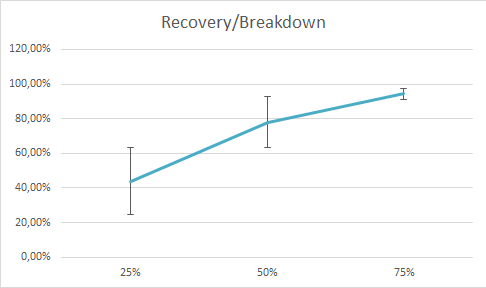
\includegraphics[width=6cm]{Figures/1.png}}
			\caption{ Recover rate for each level of knowledge}
			\label{Fig:Data1}
		\end{subfigure}
		%
		\hspace{1cm}
		%
		\begin{subfigure}[b]{0.5 \columnwidth}
			\centering
			\frame{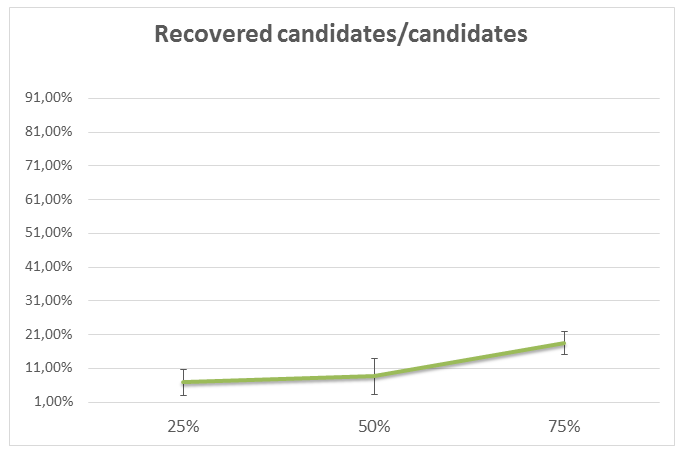
\includegraphics[width=6cm]{Figures/2.png}}
			\caption{Average number of candidates repaired for each level of knowledge}
			\label{Fig:Data2}
		\end{subfigure}
		\caption{Results for the (4, 1, 5) HTN}\label{fig:TOF2}
	\end{figure}	
	\par  Figures \ref{Fig:Data3} and  \ref{Fig:Data1} display the recover rate for HTNs calculated using the recover procedure.  We calculated the number of no null plan returned by the recover procedure for each breakdown. We notice that the hybrid system is able to propose plans recovery and switch between the procedural and the symbolic environment. Moreover, the results confirm our assumption: the graph follows a monotonic assumption in function of the symbolic knowledge. Thus, the more symbolic knowledge Discolog has the more it can recover from breakdowns. 
	
	The error bars defined in the graphs represent the standard deviations for each execution in function of the level of symbolic knowledge.  We notice that the less symbolic knowledge Discolog has the bigger is the standard deviation.  For the same HTN, Discolog gets different rates of performances. For example for HTNs defined with the 25 \% of symbolic knowledge, Discolog performances varies from  0\% to 65\%  of recover. This is noticed in the case of HTN with 25 \% and 50 \% of defined symbolic knowledge. Thus, HTNs  defined with limited symbolic domain knowledge, are unable to cover from all the possible breakdowns because of their lack of symbolic knowledge. 
	
	\par  Figures \ref{Fig:Data4} and \ref{Fig:Data2} show the average of the number of candidates repaired during the execution. Fo each list of candidates produced by the FindCandidates procedure, we calculated the number of plans produced by the recover procedure to repair them. The results for repairing  candidates also confirm our assumption. However, the error bars as demonstrated in graphs show that Discolog performances varies for repairing all the possible candidates and this independently of the level of symbolic knowledge defined. Theses result raise a new question of the quality of the symbolic knowledge defined by the designer. Symbolic knowledge is limited, then it has to be expressive and very representative of the agent policy, or Discolog will not have the precise knowledge to recover from all the possible breakdowns. 
	\par These tests are very promising but remain far from being definite experimental analysis. An extensive tests on a set of realistic domain knowledge is the object of futures works to detail the problematic of the quality of knowledge and test Discolog on real planning problems. 
	\section{Conclusion}
	\par In this paper we have presented \emph{Discolog}, an algorithm to recover from breakdowns in reactive HTN planning systems.  Despite the ability of reactive planning  to deal with high dynamic world,  breakdowns might occur because of the lack of knowledge on the different possible changes in the world and the ineptitude  of reactive HTN to reason in long term to define a recover strategy. 
	\par The proposed algorithm extends reactive HTNs with linear symbolic planner to produces a plan to recover from the breakdown. The symbolic knowledge is extracted from the procedural knowledge by the HTN designer. Thus if a breakdown is detected, the algorithm calculates the candidates (conditions which are not valid in the non-executed HTN tasks), then 
	STRIPS is called to propose plans to repair these conditions. The most promising plan is then converted to procedural formalism and executed. 
	\par The solution have been implemented. It combines a reactive HTN Disco with the symbolic linear planning system STRIPS in Prolog.  The
	results of our preliminary experiments  demonstrated, first, the ability of the hybrid planning system Discolog to propose viable plans recovery and for the different breakdowns. Second, the  contribution of symbolic knowledge in the performances of the recovery. Finally, the experiments raise another problematic of the quality of  knowledge in limited domain knowledge that we wish address. In addition, we intend to validate Discolog on real  applications such as social dialog systems, we believe that with real applications, we can study the problem of the quality of the symbolic knowledge.  
	\par Future prospects of this research are, first, to construct a modeling tool for HTN	model design. This tool will help the HTN designer in one hand to define the level of knowledge to integrate in the HTN. In the other hand, the system will use the history of breakdowns to propose adding knowledge in the HTN where breakdowns occurred. As second step, we propose to integrate Discolog in social dialog system between an agent and a human in order to support the dynamic nature of a social dialog.
	\ifCLASSOPTIONcaptionsoff
	\newpage
	\fi
	
	\label{Bibliography}
	\bibliography{Bibliography} % The references (bibliography) information are stored in the file named "Bibliography.bib"
	\bibliographystyle{ieeetr}
	
	\begin{IEEEbiography}
		\
	\end{IEEEbiography}

\end{document}

